% !TEX root=../master.tex

\chapter{Introduction}
\label{chp:introduction}

\section{Problem Statement}
As multirotor unmanned aerial vehicles (UAVs) have become extremely popular
platforms for commercial and consumer products over the past decade, a variety
of new use cases have emerged that require operation from moving vehicles.
Such use cases include
maritime surveillance, package delivery, and convoy
support (see~\figref{fig:drone_convoy_support}). While there are
many facets to operating from moving vehicles, this thesis works toward creating
a robust solution to autonomously landing multirotor UAVs onto moving vehicles
in challenging conditions.

\begin{figure}[t]
  \centering
  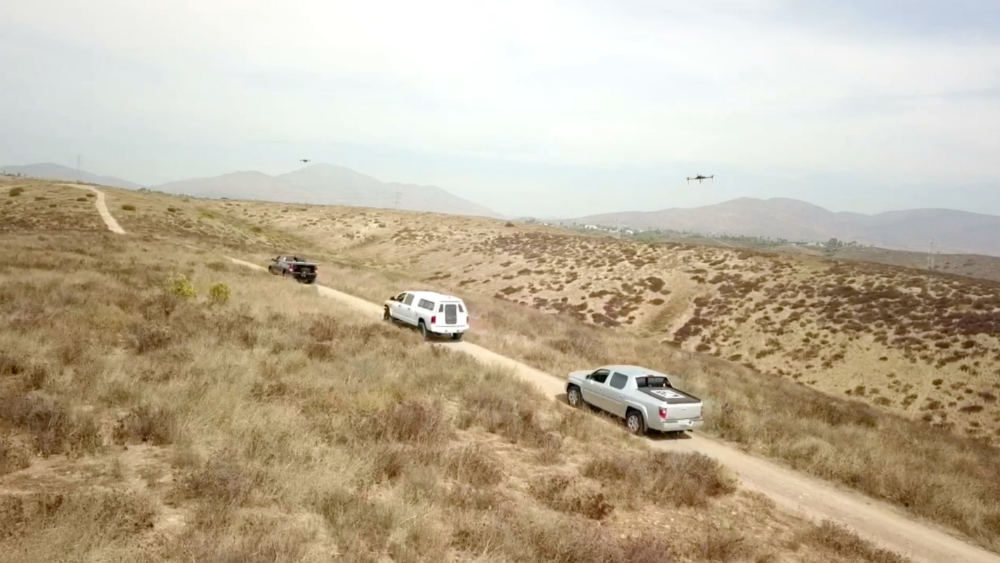
\includegraphics[width=5.5in]{figures/drone_convoy_support.png}
  \caption[UAV Convoy Support]{An example of multirotor UAVs used to increase
  situational awareness of a convoy of
vehicles~\cite{ground_vehicle_based_drones}.}
%
  \label{fig:drone_convoy_support}
\end{figure}

State-of-the-art autonomous vehicle systems require robust solutions to the
three problems of state estimation, motion planning and control. In this thesis,
we propose solutions to two of those three problems, state estimation and
control, for a multirotor UAV landing on a moving vehicle. We leave the problem
of motion planning as future work, providing some suggested direction
in~\secref{BLAH}.

\section{Background}

While autonomous landing of multirotor UAVs onto moving vehicles has been
demonstrated in a variety of scenarios~\cite{BLAH}, many problems still remain to
create a truly robust solution. Most low-cost landing methods depend on a fiducial
landing marker, such as that shown in~\figref{fig:aruco_tag}, that is rigidly attached to the landing vehicle~\cite{BLAH}.
A camera mounted to the UAV detects the fiducial landing marker, providing
information about the relative position of the UAV to the landing vehicle.
Though widely used and successful, this method quickly fails when the fiducial
landing marker is not detected for significant periods of time.

\begin{figure}[t]
  \centering
  
\includegraphics[width=2.5in]{figures/aruco_104.png}
  \caption[Visual Fiducial Landing Marker]{Visual fiducial markers such as this
    ArUco tag~\cite{garrido2016generation} are commonly used to assist in the
  landing of multirotor UAVs onto moving vehicles.}
  \label{fig:aruco_tag}
\end{figure}

\section{Contributions}

\section{Outline}
